\section{Results}
\label{sec:results}

We organize the results around five claims. First, toxic influence propagates under matched rollouts. Second, compressed memory creates a laundering effect: summaries remain classifier-clean while still shifting downstream behavior. Third, transcript and memory are distinct channels with different metric signatures. Fourth, the effect is robust across topology and injection count. Fifth, mitigation requires coordinated state and parameter controls rather than output filtering or DPO alone.

\subsection{Toxic Influence Propagates Under Matched Rollouts}
\label{sec:results_propagation}

Before analyzing laundering, we verify that upstream toxic exposure reliably changes downstream agents' behavior. This establishes the paired evaluation protocol and rules out the null hypothesis that downstream agents are insensitive to upstream tone. Across the seven primary rollout conditions, the paired effect size $\Delta\mu$ is significantly positive in every condition ($p<0.001$; full table in \Cref{tab:propagation}). Multi-injection consistently amplifies propagation relative to single-injection, while topology modulates magnitude rather than existence: chain concentrates exposure ($\Delta\mu=0.2684$), whereas high-branching fan-out dilutes the mean per-node effect ($\Delta\mu=0.0249$ under single injection). These results show that downstream toxicity is not merely the focal agent's own toxic output; it is induced in non-focal agents by the evolving conversation state.

\subsection{Memory Laundering: Classifier-Clean but Behaviorally Toxic}
\label{sec:results_laundering}

We now test the central claim: compressed memory can conceal toxic influence below classifier thresholds while preserving behavioral influence. All experiments in this subsection use the chain topology in memory-augmented mode, where downstream agents condition on the running summary $M_t$ together with the immediate parent message. Chain is the minimal setting that isolates the laundering mechanism; cross-topology validation appears in \Cref{sec:results_robustness} and \Cref{tab:tree_memory_laundering}.

\paragraph{Classifier labels say clean.}
\Cref{tab:memory_laundering} shows that toxic-condition memory summaries average $0.0852$ in Detoxify toxicity: much higher than the neutral baseline of $0.0007$, but still far below the standard filtering threshold $\tau=0.5$. Every stored memory summary in both conditions falls below threshold. Thus, a monitor applied only to the memory artifact would declare both toxic and neutral memory states safe.

\paragraph{Behavior says contaminated.}
Conditioning on those classifier-clean memories nevertheless shifts downstream behavior. Downstream responses in the toxic condition have mean toxicity $0.141$ versus $0.001$ in the matched neutral condition, giving $\mathrm{SPG}(0.5)=0.139$. The paired seed-level difference is $0.170$ with 95\% CI $[0.120,0.226]$ and Wilcoxon signed-rank $p=3.75\times10^{-8}$. \Cref{fig:spg_main} shows that SPG remains significantly positive across thresholds $\tau\in\{0.03,0.05,0.1,0.2,0.3,0.5\}$, while nearly all memory states remain below threshold. The relevant safety signal is therefore not whether $M_t$ crosses $\tau$, but whether the toxic-arm rollout continues to generate higher-toxicity downstream responses than its paired neutral rollout.

\paragraph{Mechanism.}
The qualitative pattern, illustrated in \Cref{fig:laundering_examples}, is that summarization removes explicit toxic markers while retaining adversarial framing such as condescension, conflict escalation, or us-vs-them structure. The summary looks safe to a per-artifact classifier, but the downstream model conditions on its framing and regenerates hostility. SPG captures this false-negative regime.

\begin{table}[t]
\centering
\caption{Memory laundering analysis on chain topology in memory-augmented mode with no memory sanitization. Paired toxic vs. neutral conditions use $n=200$ seeds and threshold $\tau=0.5$. Every stored memory summary falls below the classifier threshold, yet downstream behavior conditioned on classifier-clean memory diverges: $\mathbb{E}[\mathrm{tox}(v_{t+1})\mid \mathrm{tox}(M_t)<\tau,\texttt{toxic}]=0.141$ versus $0.001$ in the neutral condition.}
\label{tab:memory_laundering}
\begin{tabular}{lccc}
\toprule
Condition & Mean $\mathrm{tox}(M_t)$ & Fraction $\mathrm{tox}(M_t)<\tau$ & SPG$(\tau)$ \\
\midrule
Memory, neutral & $0.0007$ & $1.00$ & -- \\
Memory, toxic   & $0.0852$ & $1.00$ & $0.139$ \\
\bottomrule
\end{tabular}
\end{table}
\begin{figure}[t]
\centering
\begin{minipage}{0.55\linewidth}
  \centering
  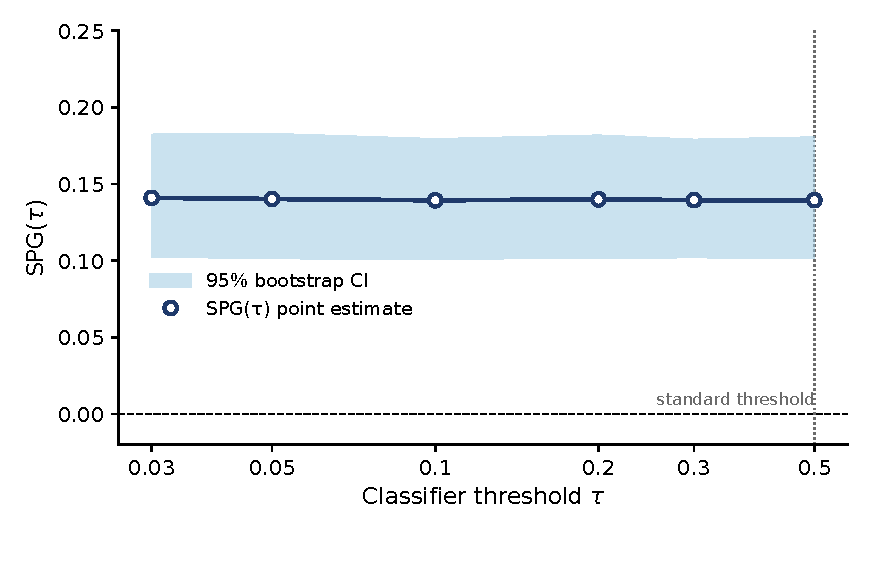
\includegraphics[width=\linewidth]{figs/spg_vs_threshold.pdf}
\end{minipage}\hfill
\begin{minipage}{0.4\linewidth}
  \caption{\textbf{Sub-threshold propagation gap.}
  SPG$(\tau)$ as a function of classifier threshold under memory-augmented chain rollouts.
  SPG remains stable at approximately $0.17$ across $\tau\in\{0.03,0.05,0.1,0.2,0.3,0.5\}$ and is positive at every threshold (all $p<0.001$, paired Wilcoxon).
  The shaded band shows the 95\% bootstrap CI.}
  \label{fig:spg_main}
\end{minipage}
\end{figure}

\subsection{Transcript and Memory are Distinct Propagation Channels}
\label{sec:results_channels}

We next disentangle which state channel carries the propagation signal. Transcript-only modes disable memory and expose downstream agents either to the full transcript or to the immediate parent. Memory-only mode exposes downstream agents only to the compressed summary $M_t$. Combined-channel mode activates both. We also evaluate memory-side interventions after compression and transcript-side write gates before compression.

\paragraph{Transcript dominates overt propagation.}
As shown in \Cref{tab:channel_comparison}, full-transcript exposure yields $\Delta\mu=0.2684$, parent-only transcript exposure yields $\Delta\mu=0.1657$, and memory-only exposure yields only $\Delta\mu=0.0115$. The combined-channel condition yields $\Delta\mu=0.1678$, nearly identical to parent-only transcript exposure. Overt downstream toxicity is therefore primarily a transcript-backflow phenomenon.

\paragraph{Memory dominates hidden influence.}
The SPG pattern is different. Memory-only mode has small visible propagation ($\Delta\mu=0.0115$) but large hidden influence ($\mathrm{SPG}=0.0970$), despite low mean memory toxicity. This is exactly the laundering regime: compressed memory does not strongly raise the average downstream toxicity metric, but it shifts the toxic-arm distribution among states a classifier labels clean.

\paragraph{Order of operations determines whether laundering is closed.}
Memory-side rewriting and gating, applied after compression, reduce $\Delta\mu$ but leave SPG high: $0.0856$ and $0.1030$, respectively. Transcript-side write gates, applied before toxic content enters the transcript or memory update, reduce both $\Delta\mu$ and SPG to near zero. Sanitization after compression is therefore too late for threshold-triggered defenses; sanitization before compression blocks the source signal before it is laundered.

\begin{table}[t]
\centering
\small
\setlength{\tabcolsep}{3pt}
\caption{Channel comparison between transcript and memory modes on chain topology at $\tau=0.5$. Transcript visibility drives overt propagation measured by $\Delta\mu$, while compressed memory carries the hidden sub-threshold signal measured by SPG.}
\label{tab:channel_comparison}
\begin{tabular}{lcccc}
\toprule
Mode / intervention & Mean tox($M_t$) & $\Delta\mu$ & SPG($\tau$=0.5) & Final tox \\
\midrule
Full transcript (no memory)              & --     & 0.2684 & --     & 0.1425 \\
Parent-only transcript (no memory)       & --     & 0.1657 & --     & 0.0173 \\
Memory only (no parent)                  & 0.0144 & 0.0115 & 0.0970 & 0.0325 \\
Memory, no sanitization (both channels)  & 0.0852 & 0.1678 & 0.1395 & 0.1470 \\
Memory + rewrite ($\tau=0.5$)            & 0.0121 & 0.0244 & 0.0856 & 0.0445 \\
Memory + gate ($\tau=0.5$)               & 0.0142 & 0.0413 & 0.1030 & 0.0146 \\
Write-gate redact ($\tau=0.5$)           & 0.0126 & 0.0031 & 0.0004 & 0.0255 \\
Write-gate rewrite ($\tau=0.5$)          & 0.0147 & 0.0069 & 0.0006 & 0.0154 \\
\bottomrule
\end{tabular}
\end{table}

\subsection{Robustness Across Topology and Injection Count}
\label{sec:results_robustness}

The propagation and laundering effects are not restricted to a single graph shape. The full robustness table in \Cref{tab:propagation} shows positive $\Delta\mu$ across chain, tree, DAG, and high-branching topologies, with multi-injection consistently increasing the effect relative to single injection. Topology changes the geometry: chains concentrate exposure, high-branching graphs dilute mean toxicity across many parallel replies, and multi-injection produces stronger persistence.

We also replicate the memory-laundering experiment on tree topology (\Cref{tab:tree_memory_laundering}). The magnitude is smaller than in the chain setting, but SPG remains significantly positive ($\mathrm{SPG}=0.0492$, $p<0.001$). This is the setting where SPG is most useful diagnostically: overt propagation is small enough that a mean-based evaluation could conclude the risk is attenuated, while the sub-threshold contrast still reveals hidden influence in classifier-clean memory.

\subsection{Defense Comparison and Full Ablation}
\label{sec:results_defense_ablation}

The preceding results show that toxic influence persists through two state channels: an overt transcript channel captured by $\Delta\mu$, and a compressed-memory channel captured by SPG. We now compare standard defenses with channel-aware interventions. This provides baselines and tests the design claim from \S\ref{sec:objective}: defenses that act only on outputs or parameters are incomplete when agents repeatedly condition on contaminated transcript and memory state.

\paragraph{Conditions.}
We evaluate nine conditions on \texttt{Llama-3.1-8B-Instruct} chain memory rollouts. The baselines are no intervention, output filtering, and DPO only. Output filtering replaces any generated message with $\mathrm{tox}(v)>\tau$ by a fixed neutral placeholder before it is appended to the transcript. The single-channel interventions are transcript-only write-gate rewriting and memory-only rewriting. The combination conditions are Transcript + Memory, Transcript + DPO, Memory + DPO, and the Full system. All conditions use $n=200$ paired seeds, single injection at $A_1$, and the chain depth-4 memory protocol.

\begin{table*}[t]
\centering
\caption{Unified comparison of baselines, single-channel interventions, and full-system combinations on \texttt{Llama-3.1-8B-Instruct} chain memory rollouts ($n=200$ paired seeds per condition). Transcript and memory controls use rewrite sanitization at $\tau=0.5$. Values are mean $\pm$ standard error. Bold marks the lowest value in each column.}
\vspace{5pt}
\label{tab:defense_ablation}
\begin{tabular}{lccc}
\toprule
Condition & Turn-4 tox & $\Delta\mu$ & SPG($\tau{=}0.5$) \\
\midrule
\multicolumn{4}{l}{\textit{Baselines}} \\
No intervention      & 0.1207 $\pm$ 0.012 & 0.1302 $\pm$ 0.015 & 0.0149 $\pm$ 0.008 \\
Output filter        & 0.0204 $\pm$ 0.004 & 0.0608 $\pm$ 0.010 & 0.0143 $\pm$ 0.004 \\
DPO only             & 0.0601 $\pm$ 0.009 & 0.0605 $\pm$ 0.012 & 0.0086 $\pm$ 0.006 \\
\midrule
\multicolumn{4}{l}{\textit{Single-channel interventions}} \\
Transcript only      & 0.0305 $\pm$ 0.006 & 0.0309 $\pm$ 0.007 & 0.0053 $\pm$ 0.003 \\
Memory only          & 0.0804 $\pm$ 0.011 & 0.0807 $\pm$ 0.013 & 0.0027 $\pm$ 0.002 \\
\midrule
\multicolumn{4}{l}{\textit{Combinations}} \\
Transcript + Memory  & 0.0202 $\pm$ 0.004 & 0.0108 $\pm$ 0.004 & \textbf{0.0012 $\pm$ 0.001} \\
Transcript + DPO     & 0.0154 $\pm$ 0.003 & 0.0159 $\pm$ 0.004 & 0.0036 $\pm$ 0.002 \\
Memory + DPO         & 0.0402 $\pm$ 0.007 & 0.0407 $\pm$ 0.008 & 0.0018 $\pm$ 0.001 \\
Full system          & \textbf{0.0106 $\pm$ 0.002} & \textbf{0.0059 $\pm$ 0.003} & 0.0014 $\pm$ 0.001 \\
\bottomrule
\end{tabular}
\end{table*}

\paragraph{Output filtering suppresses visible toxicity but not propagation.}
The output filter lowers turn-4 toxicity from $0.1207$ to $0.0204$, showing that it blocks many overtly toxic generations. However, $\Delta\mu$ remains $0.0608$, and SPG is essentially unchanged ($0.0149$ to $0.0143$). The filter therefore improves the visible final message while leaving a substantial toxic-neutral trajectory gap and the laundered memory pathway intact.

\paragraph{DPO reduces amplification but does not clean the state.}
DPO-only reduces $\Delta\mu$ from $0.1302$ to $0.0605$ and SPG from $0.0149$ to $0.0086$. This confirms that parameter-level intervention is useful. But DPO does not remove toxic transcript or compressed memory from future contexts, so the agent is still repeatedly conditioned on contaminated state. DPO is therefore complementary to state control, not a replacement for it.

\paragraph{Single-channel controls expose transcript-memory asymmetry.}
Transcript-only control reduces $\Delta\mu$ to $0.0309$, whereas memory-only control leaves $\Delta\mu=0.0807$. Conversely, memory-only control gives the strongest single-channel SPG reduction ($0.0027$), consistent with SPG measuring hidden memory influence rather than overt transcript backflow. Neither single-channel intervention is sufficient: transcript control leaves residual memory-mediated influence, and memory control leaves transcript backflow intact.

\paragraph{Combinations show that the channels are complementary.}
Transcript + Memory reduces $\Delta\mu$ to $0.0108$ and SPG to $0.0012$, showing that direct state control over both transcript and memory removes most of the propagation signal even without DPO. Adding DPO to Transcript-only and Memory-only further reduces $\Delta\mu$ to $0.0159$ and $0.0407$, respectively, suggesting that DPO reduces residual amplification after whichever state channels remain active.

\paragraph{Takeaway.}
The full system achieves the lowest turn-4 toxicity ($0.0106$) and lowest overall propagation gap ($\Delta\mu=0.0059$), while maintaining near-minimal SPG ($0.0014$). The ablation supports the multi-pathway design: transcript control suppresses overt backflow, memory control suppresses sub-threshold laundering, and DPO reduces residual model-level amplification. Output filtering and DPO alone each reduce part of the problem, but neither removes contaminated state from the conditioning loop.

\begin{comment}\section{Results}
\label{sec:results}

We organize results into two parts: \emph{phenomenon} results establishing that toxic backflow is a real and measurable effect (\S\ref{sec:p_results}--\S\ref{sec: propagation}), and \emph{intervention} results demonstrating the necessity of multi-pathway unlearning (\S\ref{subsec:state_ablation}--\S\ref{subsec:full_ablation}).

\subsection{Main Phenomenon Results}
\label{sec:p_results}
%-------------------------------------------------------------

\paragraph{Finding: Toxic injection causes immediate, significant
propagation across all topology conditions.}
All seven conditions yield statistically significant positive effect
sizes ($\Delta\mu > 0$, Wilcoxon $p \leq 0.008$; Figure~\ref{fig:delta_mu}).
Single-injection conditions produce mean $\Delta\mu \approx 0.12$--$0.13$;
multi-injection conditions produce mean $\Delta\mu \approx 0.38$,
a roughly $3\times$ amplification.
Under the \emph{neutral} condition, Detoxify scores remain near
zero across all topologies (mean max toxicity $\leq 0.003$),
confirming that elevated toxicity in paired graphs is attributable
solely to $\text{A}_1$'s policy.

%-------------------------------------------------------------
\subsection{Context Visibility Ablation}
\label{sec:context_ablation}
%-------------------------------------------------------------
To isolate the propagation mechanism, we vary what downstream agents can observe (Table~\ref{tab:context_ablation}).

Comparing \emph{tree--single} (full-visible context) against
\emph{tree--single--parent-only} (parent-only context) isolates
the contribution of transcript backflow to propagation.
Mean $\Delta\mu$ is essentially identical across the two conditions
($0.130$ vs.\ $0.123$; $p = 0.008$ for parent-only vs.\
$p < 0.001$ for full-visible), indicating that even minimal context
exposure---one parent message---is sufficient to sustain significant
toxic propagation.
However, the relay amplification at $k=2$ observed under full-visible
context is dampened under parent-only, and the variance of
$\Delta\mu$ is higher under parent-only (wider CI in
Figure~\ref{fig:delta_mu}), consistent with reduced but noisier
propagation when downstream context is restricted.
This pattern motivates read-side sanitization as an intervention:
if even one contaminated parent message is sufficient to induce
propagation, sanitizing the context window before each generation
step is a necessary (though possibly not sufficient) mitigation.

\begin{table}[t]
\centering
\caption{Context ablation on chain topology ($N=200$ seeds). Mean toxicity at turn~4 under strong $A_1$. $\Delta$ denotes the paired effect size (toxic $-$ neutral).}
\label{tab:context_ablation}
\small
\begin{tabular}{lcc}
\toprule
Context mode & Mean tox (turn 4) & $\Delta\mu$ \\
\midrule
Full transcript  & \texttt{[--]} & \texttt{[--]} \\
Parent-only      & \texttt{[--]} & \texttt{[--]} \\
Seed-only        & \texttt{[--]} & \texttt{[--]} \\
\bottomrule
\end{tabular}
\end{table}

\paragraph{Key finding.}
The full-transcript condition produces the largest downstream toxicity effect, while the seed-only condition (where agents see only the original post) produces near-zero propagation.
This confirms that toxic backflow---the mechanism by which toxic content persists in the conditioning state and re-enters the agent's context at each turn---is the dominant propagation channel, rather than intrinsic model bias or seed-level priming.


% ============================================================
%  Figure reference stubs — update labels to match yours
% ============================================================

 \begin{figure}[t]
   \centering
   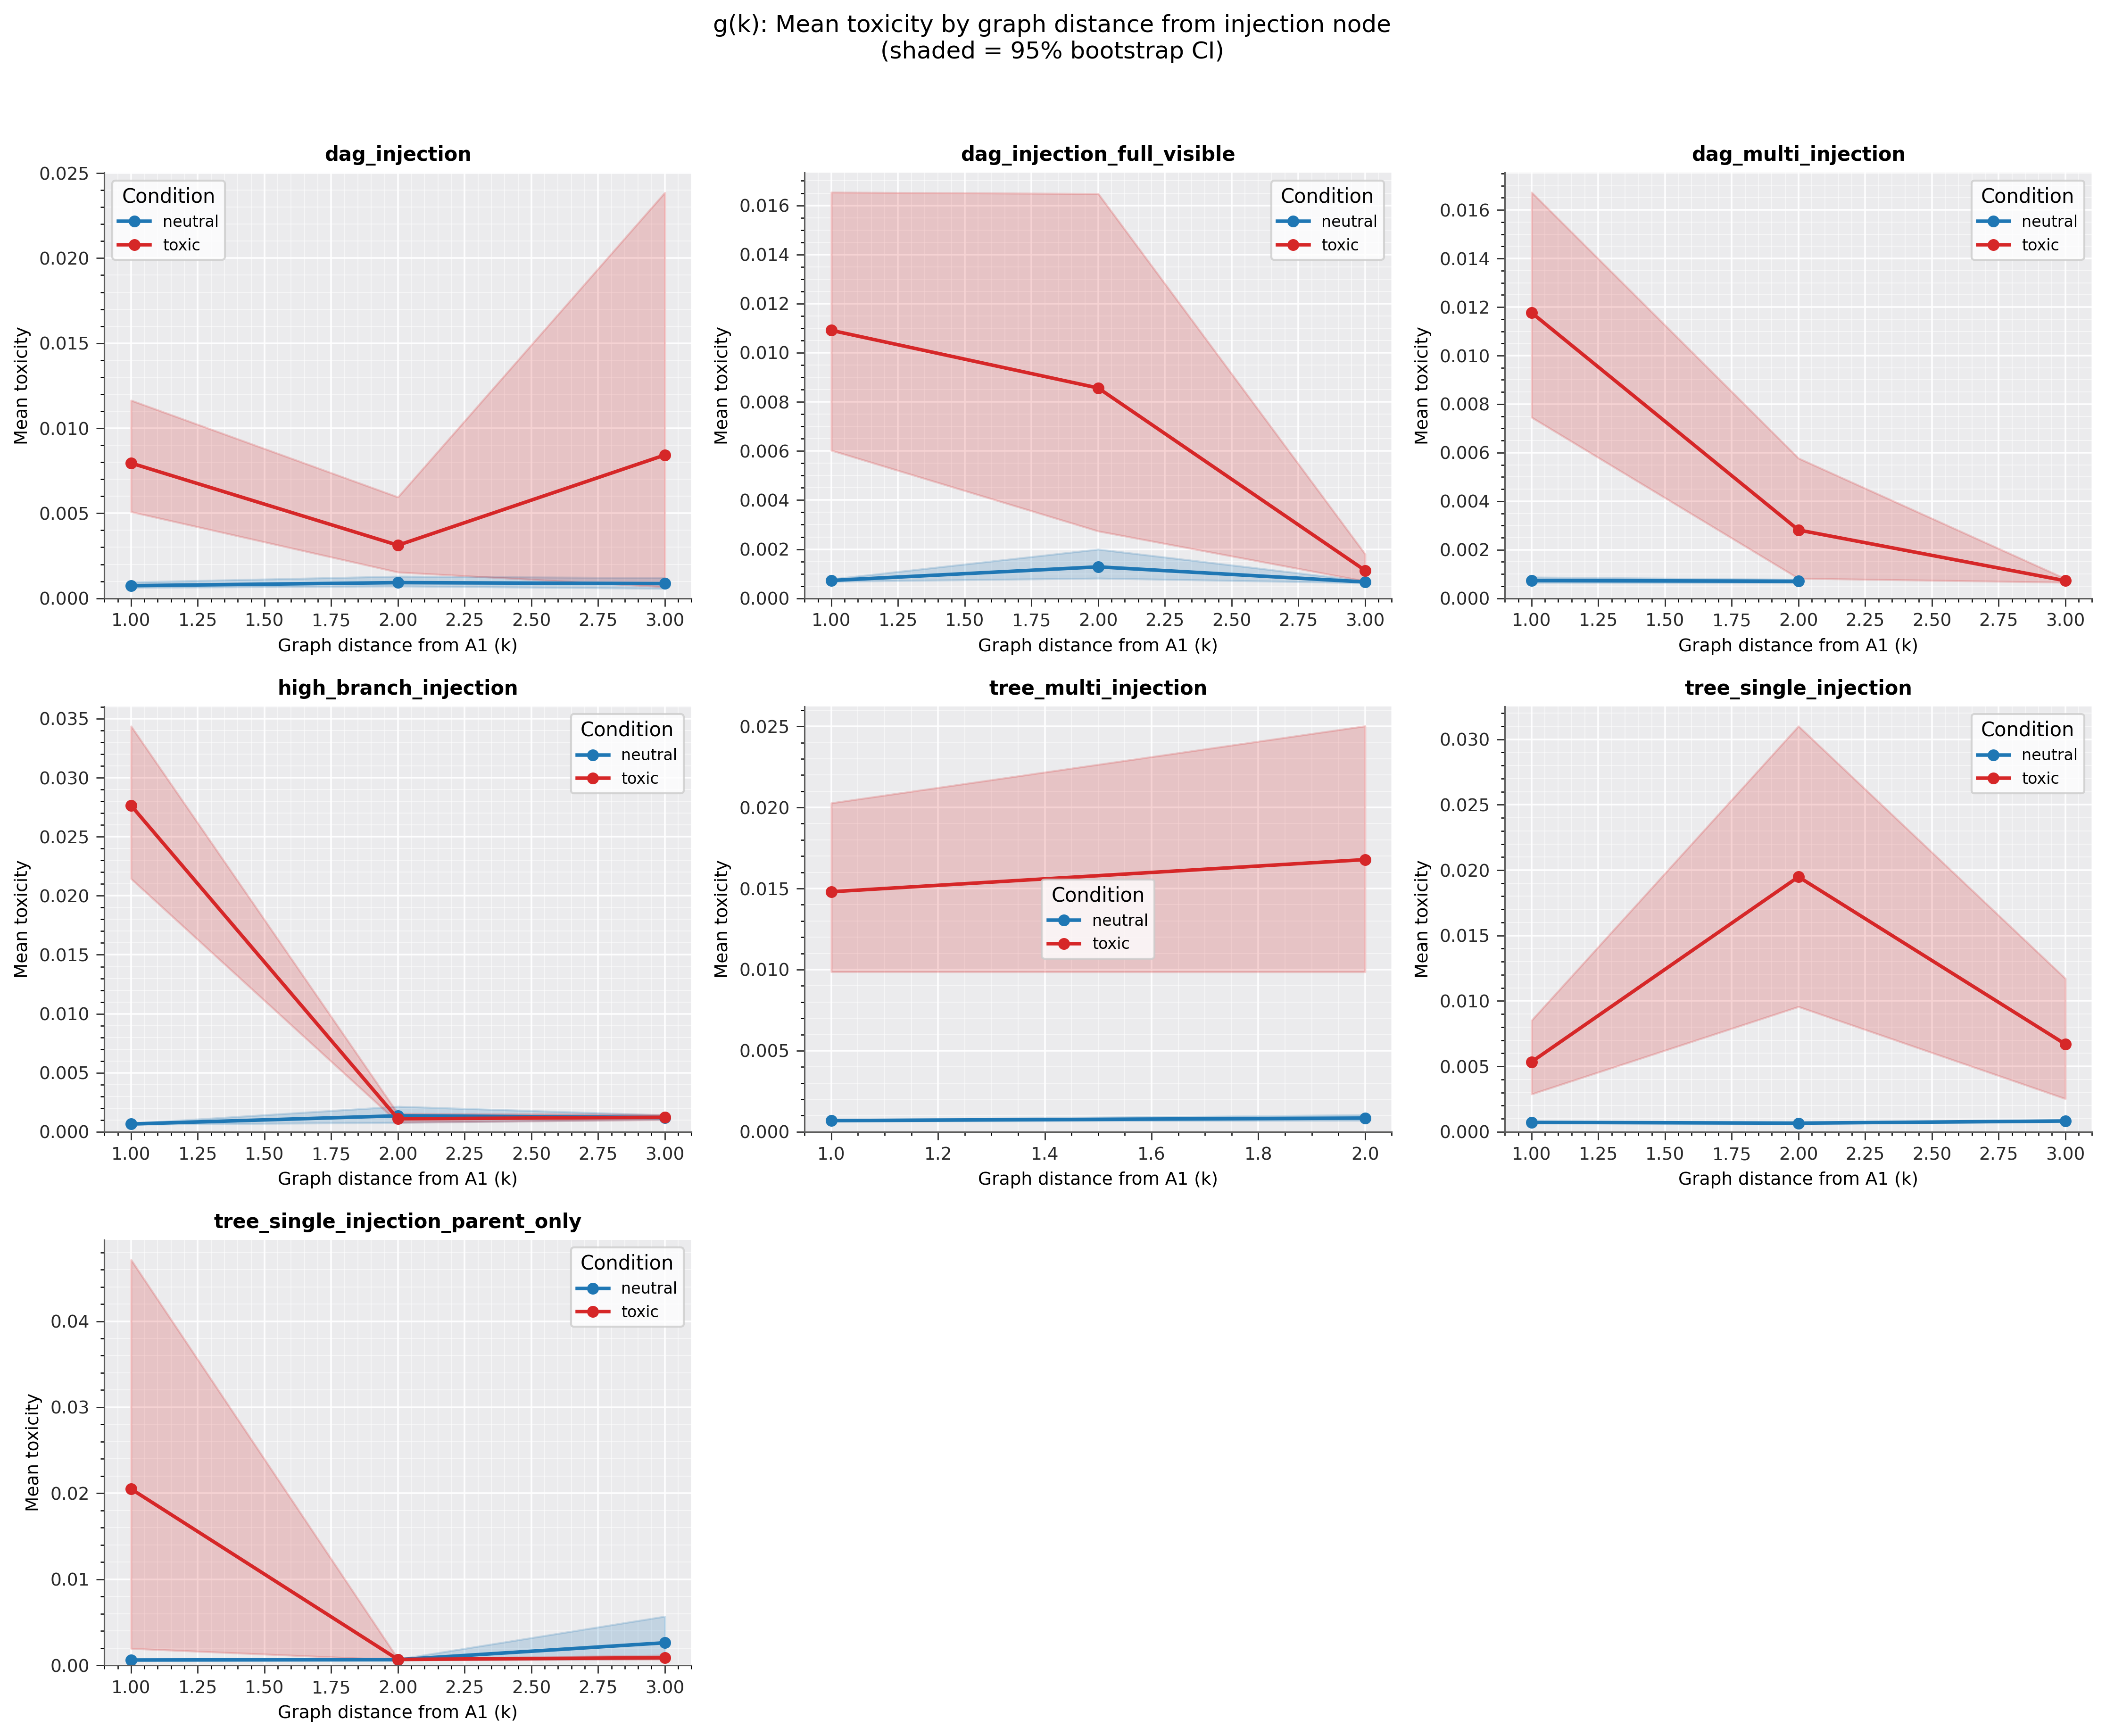
\includegraphics[width=\linewidth]{figs/g_k_propagation_radius.png}
   \caption{$g(k)$: mean toxicity by graph distance from the injection
   node $\text{A}_1$ (shaded = 95\% bootstrap CI).  Toxicity attenuates
   with distance in most conditions; tree topologies exhibit a relay
   amplification at $k=2$ under full-visible context.}
   \label{fig:gk}
 \end{figure}

 \begin{figure}[t]
   \centering
   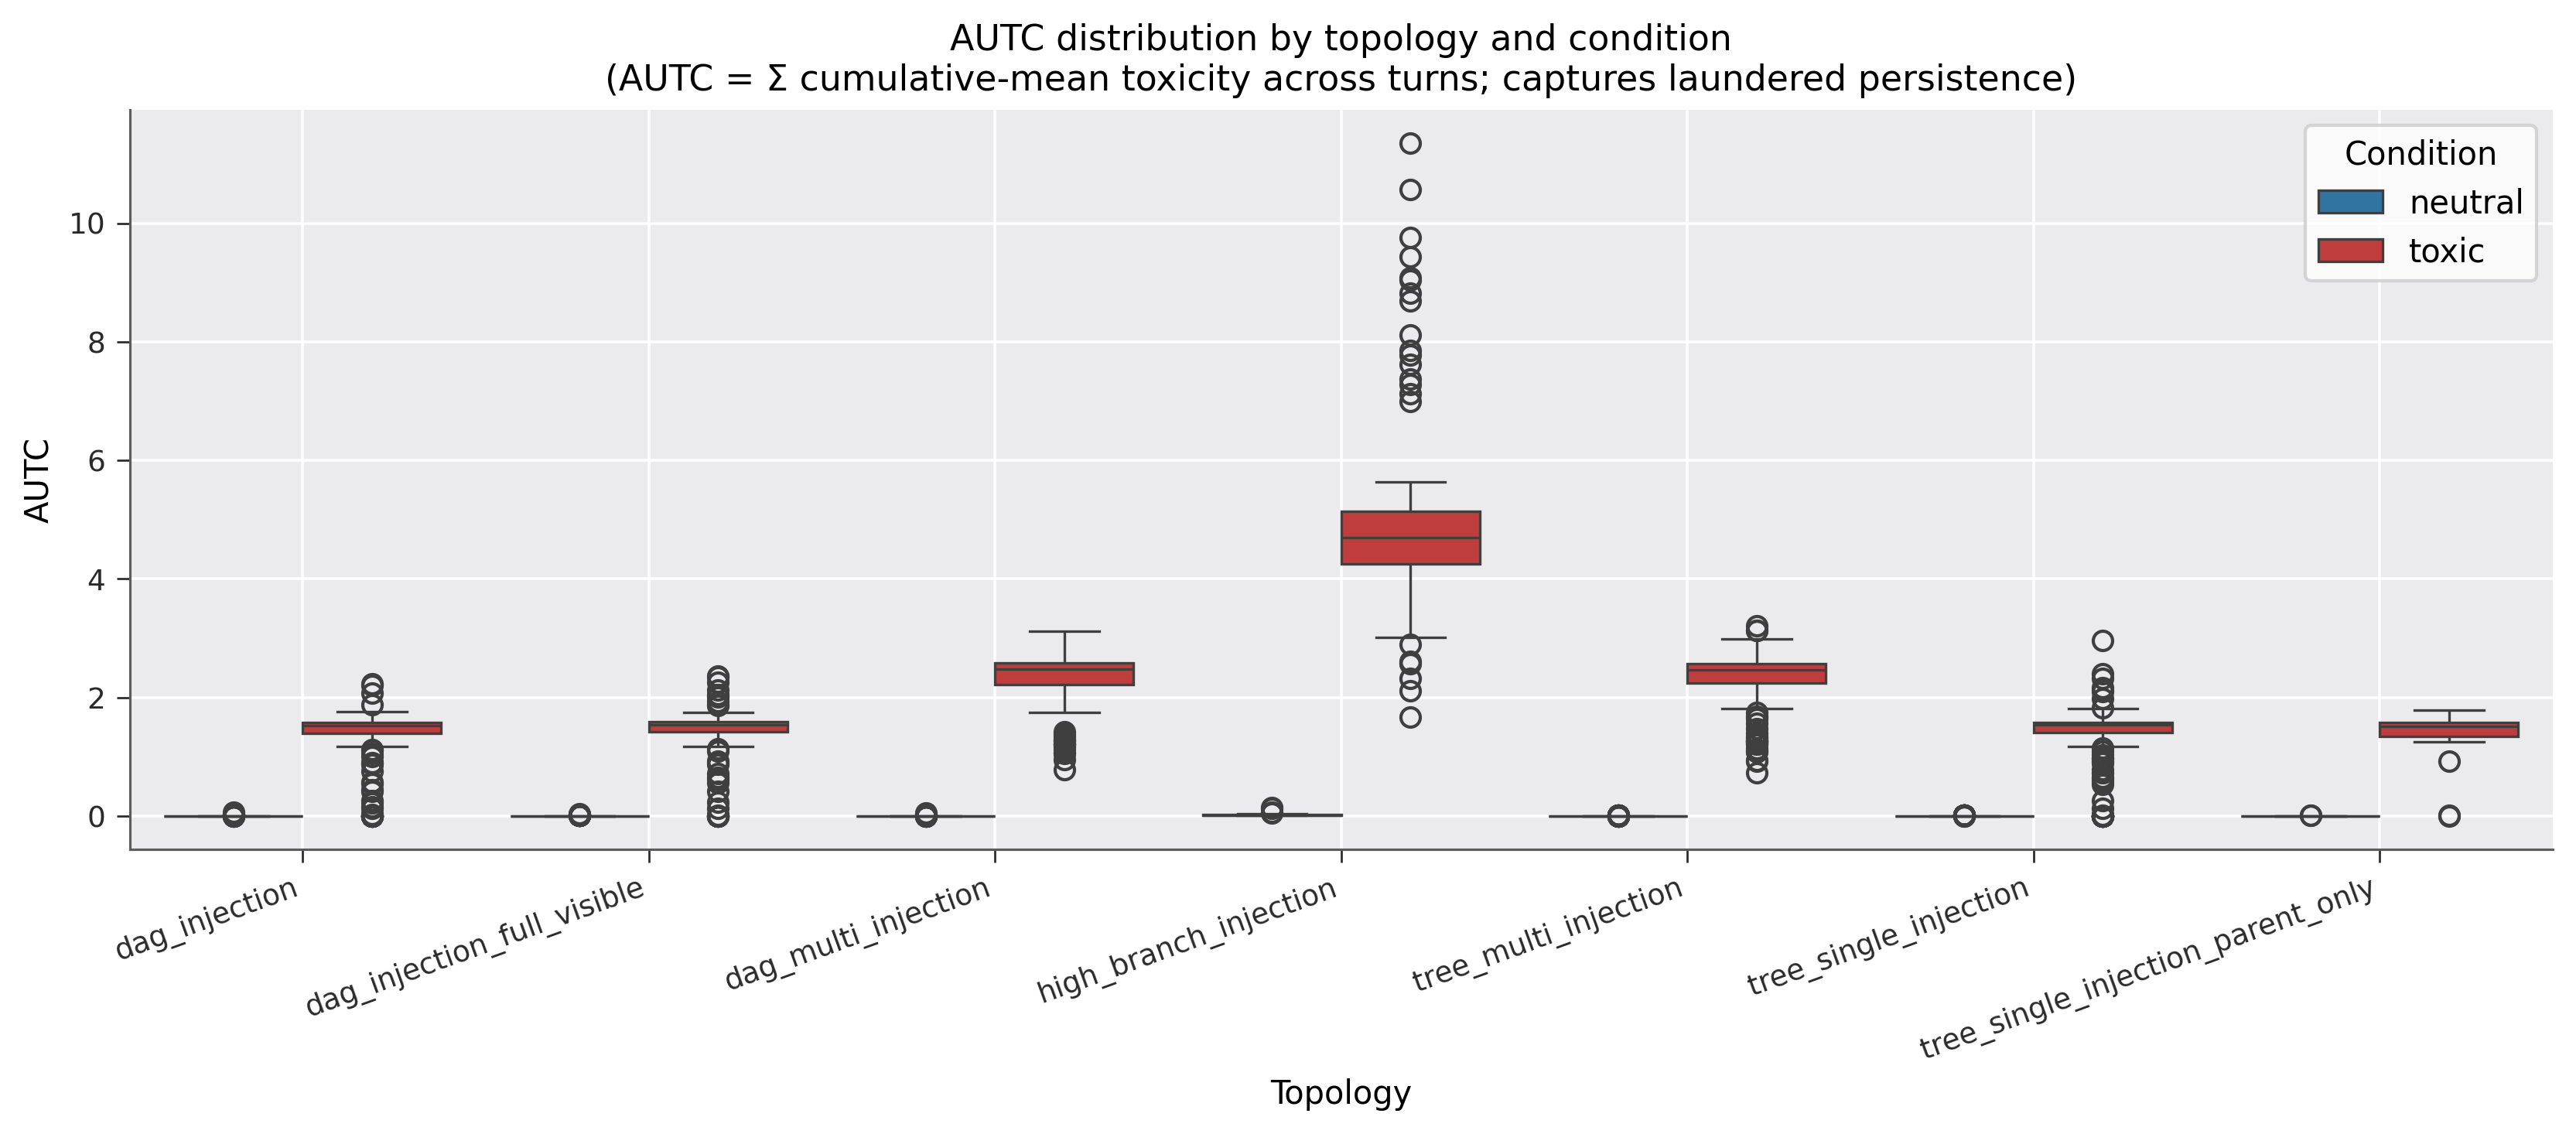
\includegraphics[width=\linewidth]{figs/autc_distribution.png}
   \caption{AUTC ($= \sum_t \mu_t$, area under the cumulative-mean
   toxicity curve) by topology and condition.  Neutral threads collapse
   to ${\approx}0$ in all conditions.  Under multi-injection,
   \emph{tree--multi} reaches median AUTC ${\approx}4.8$ with a long
   upper tail, capturing the laundered-toxicity regime where toxic
   framing recurs below per-turn classifier thresholds.}
   \label{fig:autc}
 \end{figure}

 \begin{figure}[t]
   \centering
   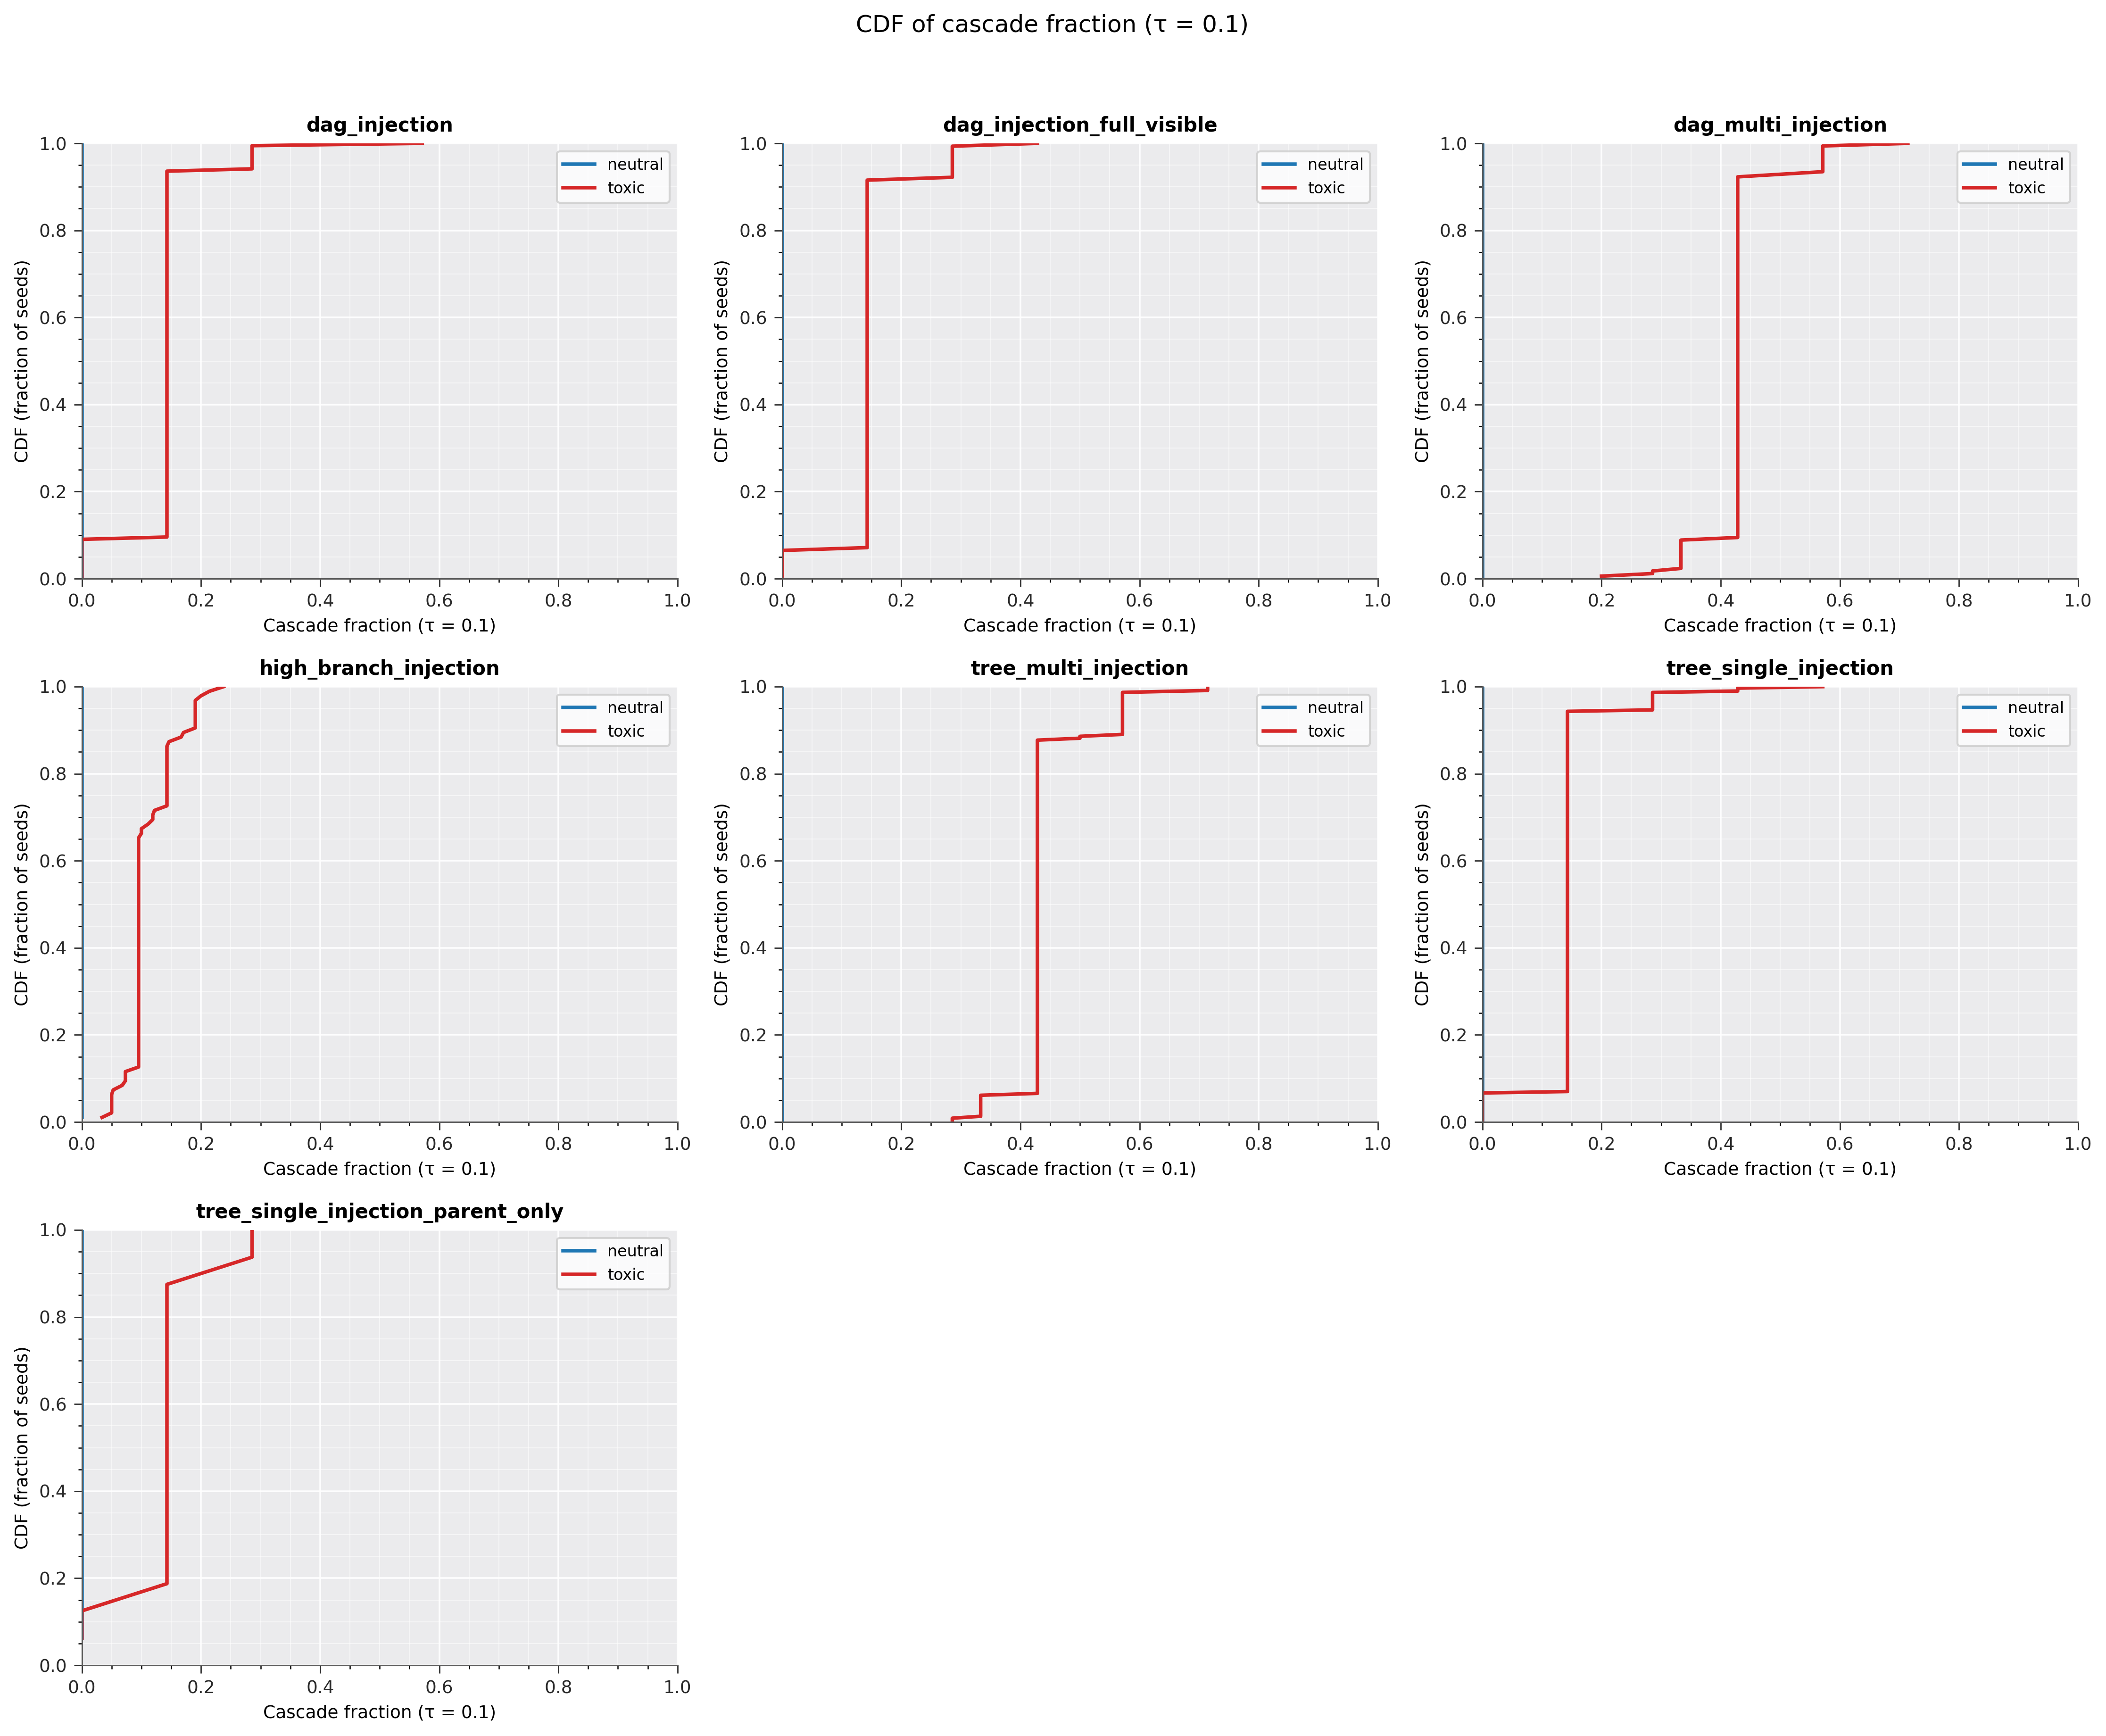
\includegraphics[width=\linewidth]{figs/cascade_fraction_cdf.png}
   \caption{CDF of cascade fraction $p_\tau(G)$ ($\tau = 0.1$) across
   seeds.  Neutral conditions concentrate at cascade fraction ${\approx}0$
   in all panels.  Multi-injection and high-branch conditions produce
   flatter toxic CDFs (wider cascade spread), while single-injection DAG
   concentrates toxic cascades below 20\%.}
   \label{fig:cascade}
 \end{figure}

 \begin{figure}[t]
   \centering
   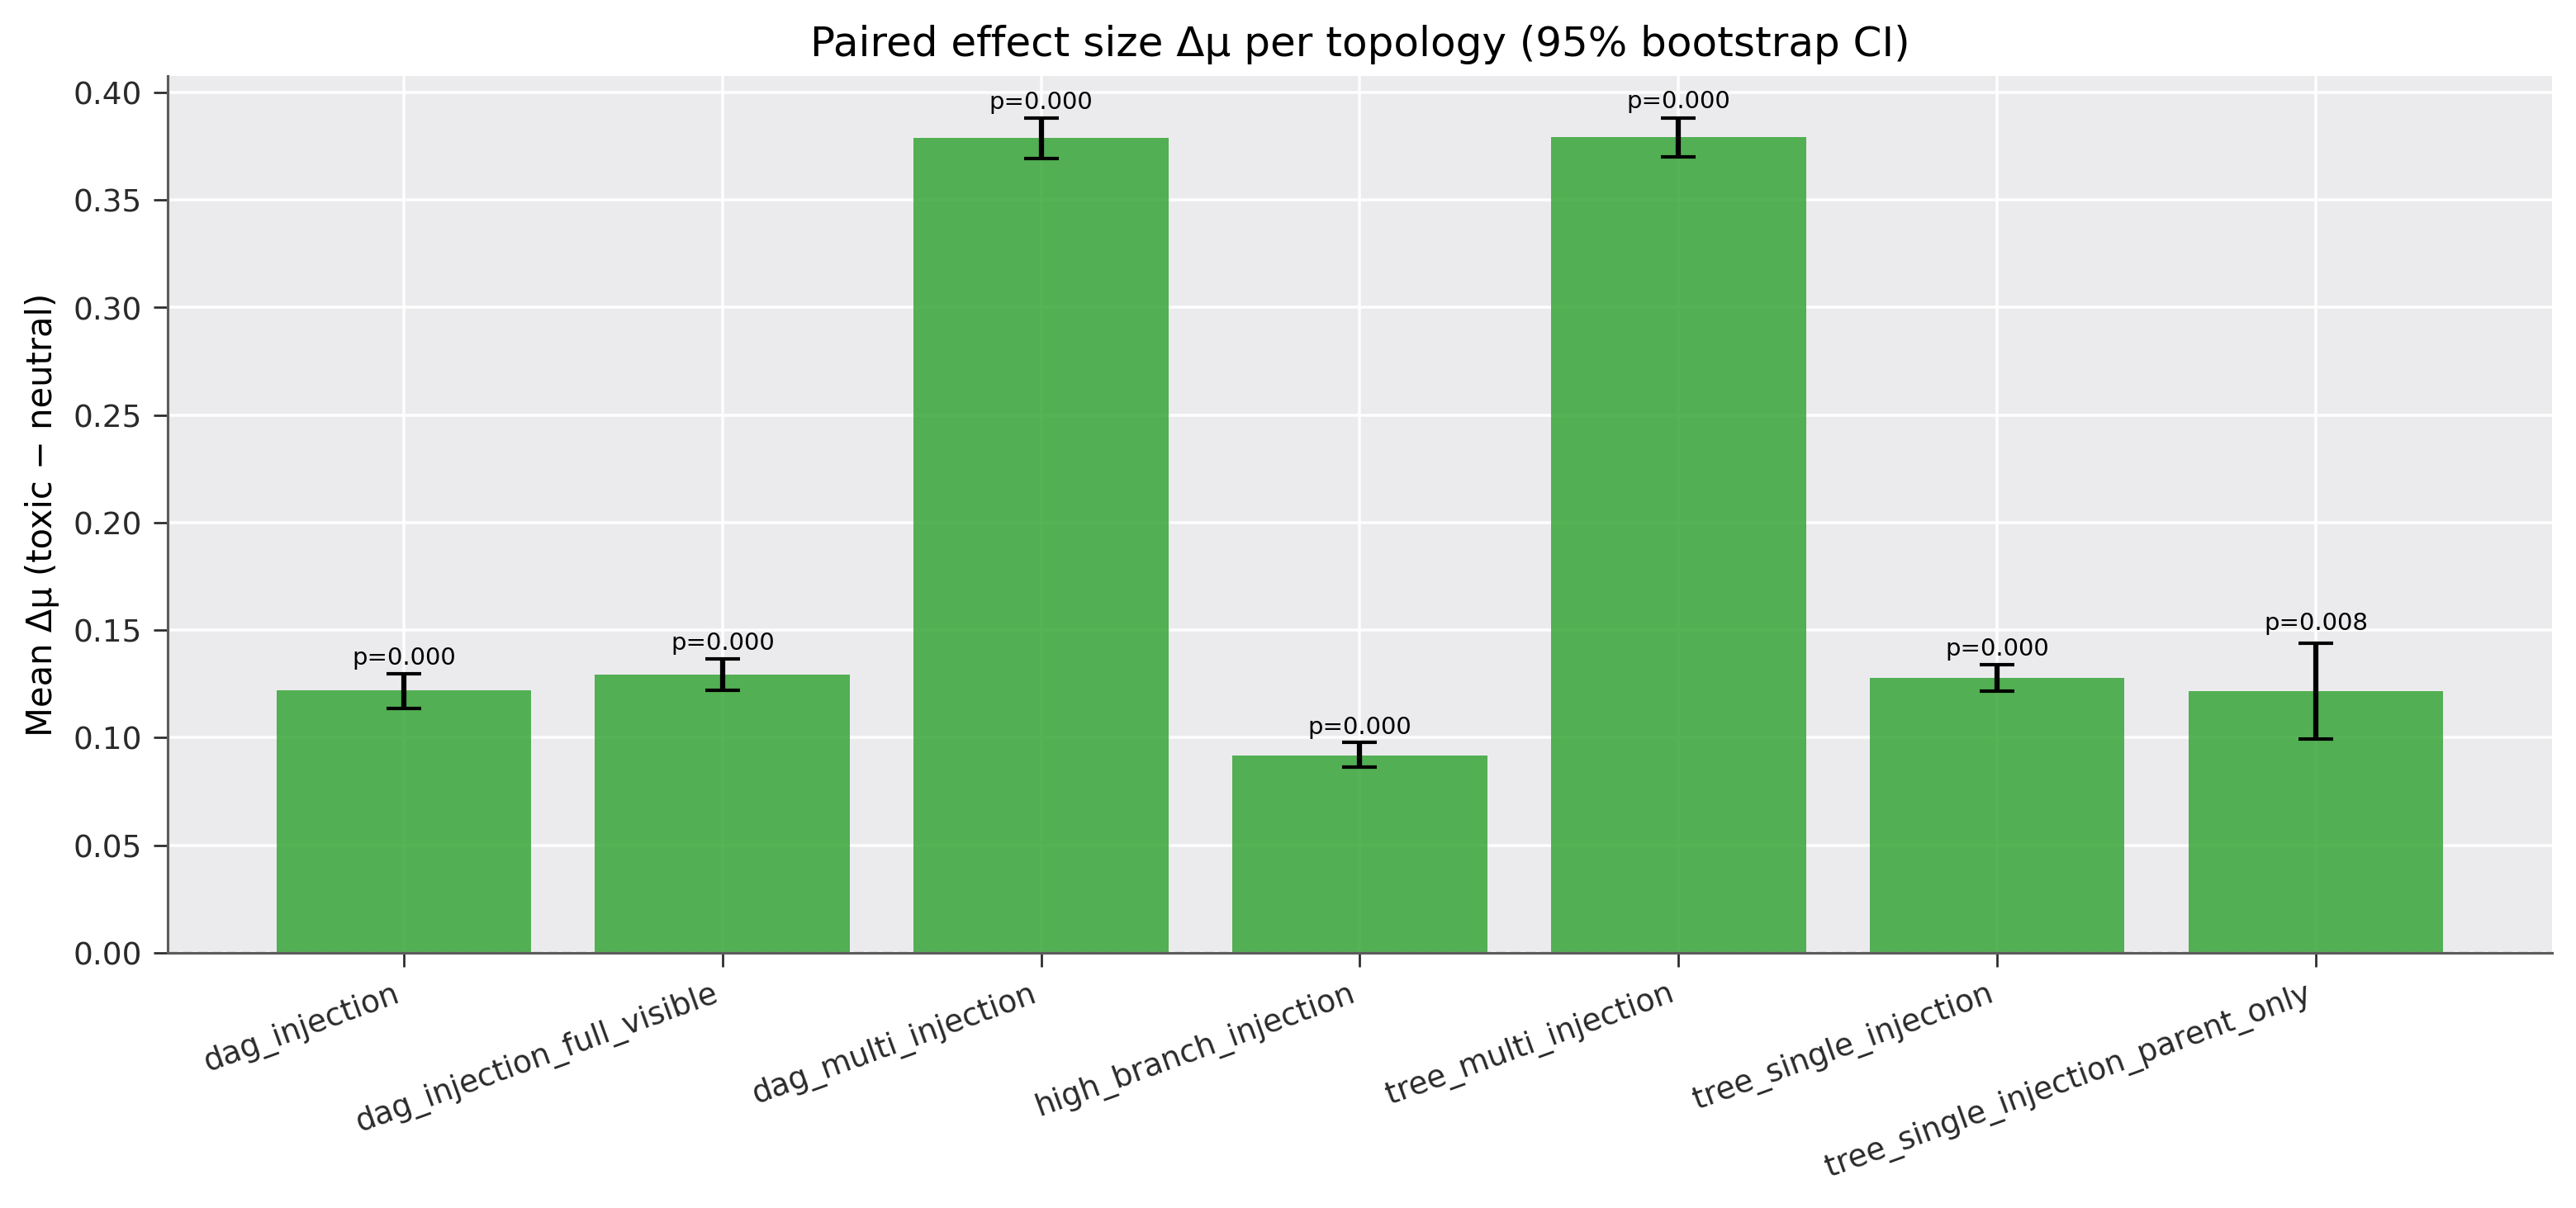
\includegraphics[width=\linewidth]{figs/paired_effect_size.png}
   \caption{Paired effect size $\Delta\mu(s)$ per topology (95\%
   bootstrap CI; Wilcoxon $p$-values annotated).  Multi-injection
   conditions (tree and DAG) reach $\Delta\mu \approx 0.38$,
   approximately $3\times$ the single-injection baseline.}
   \label{fig:delta_mu}
 \end{figure}

 \begin{figure}[t]
   \centering
   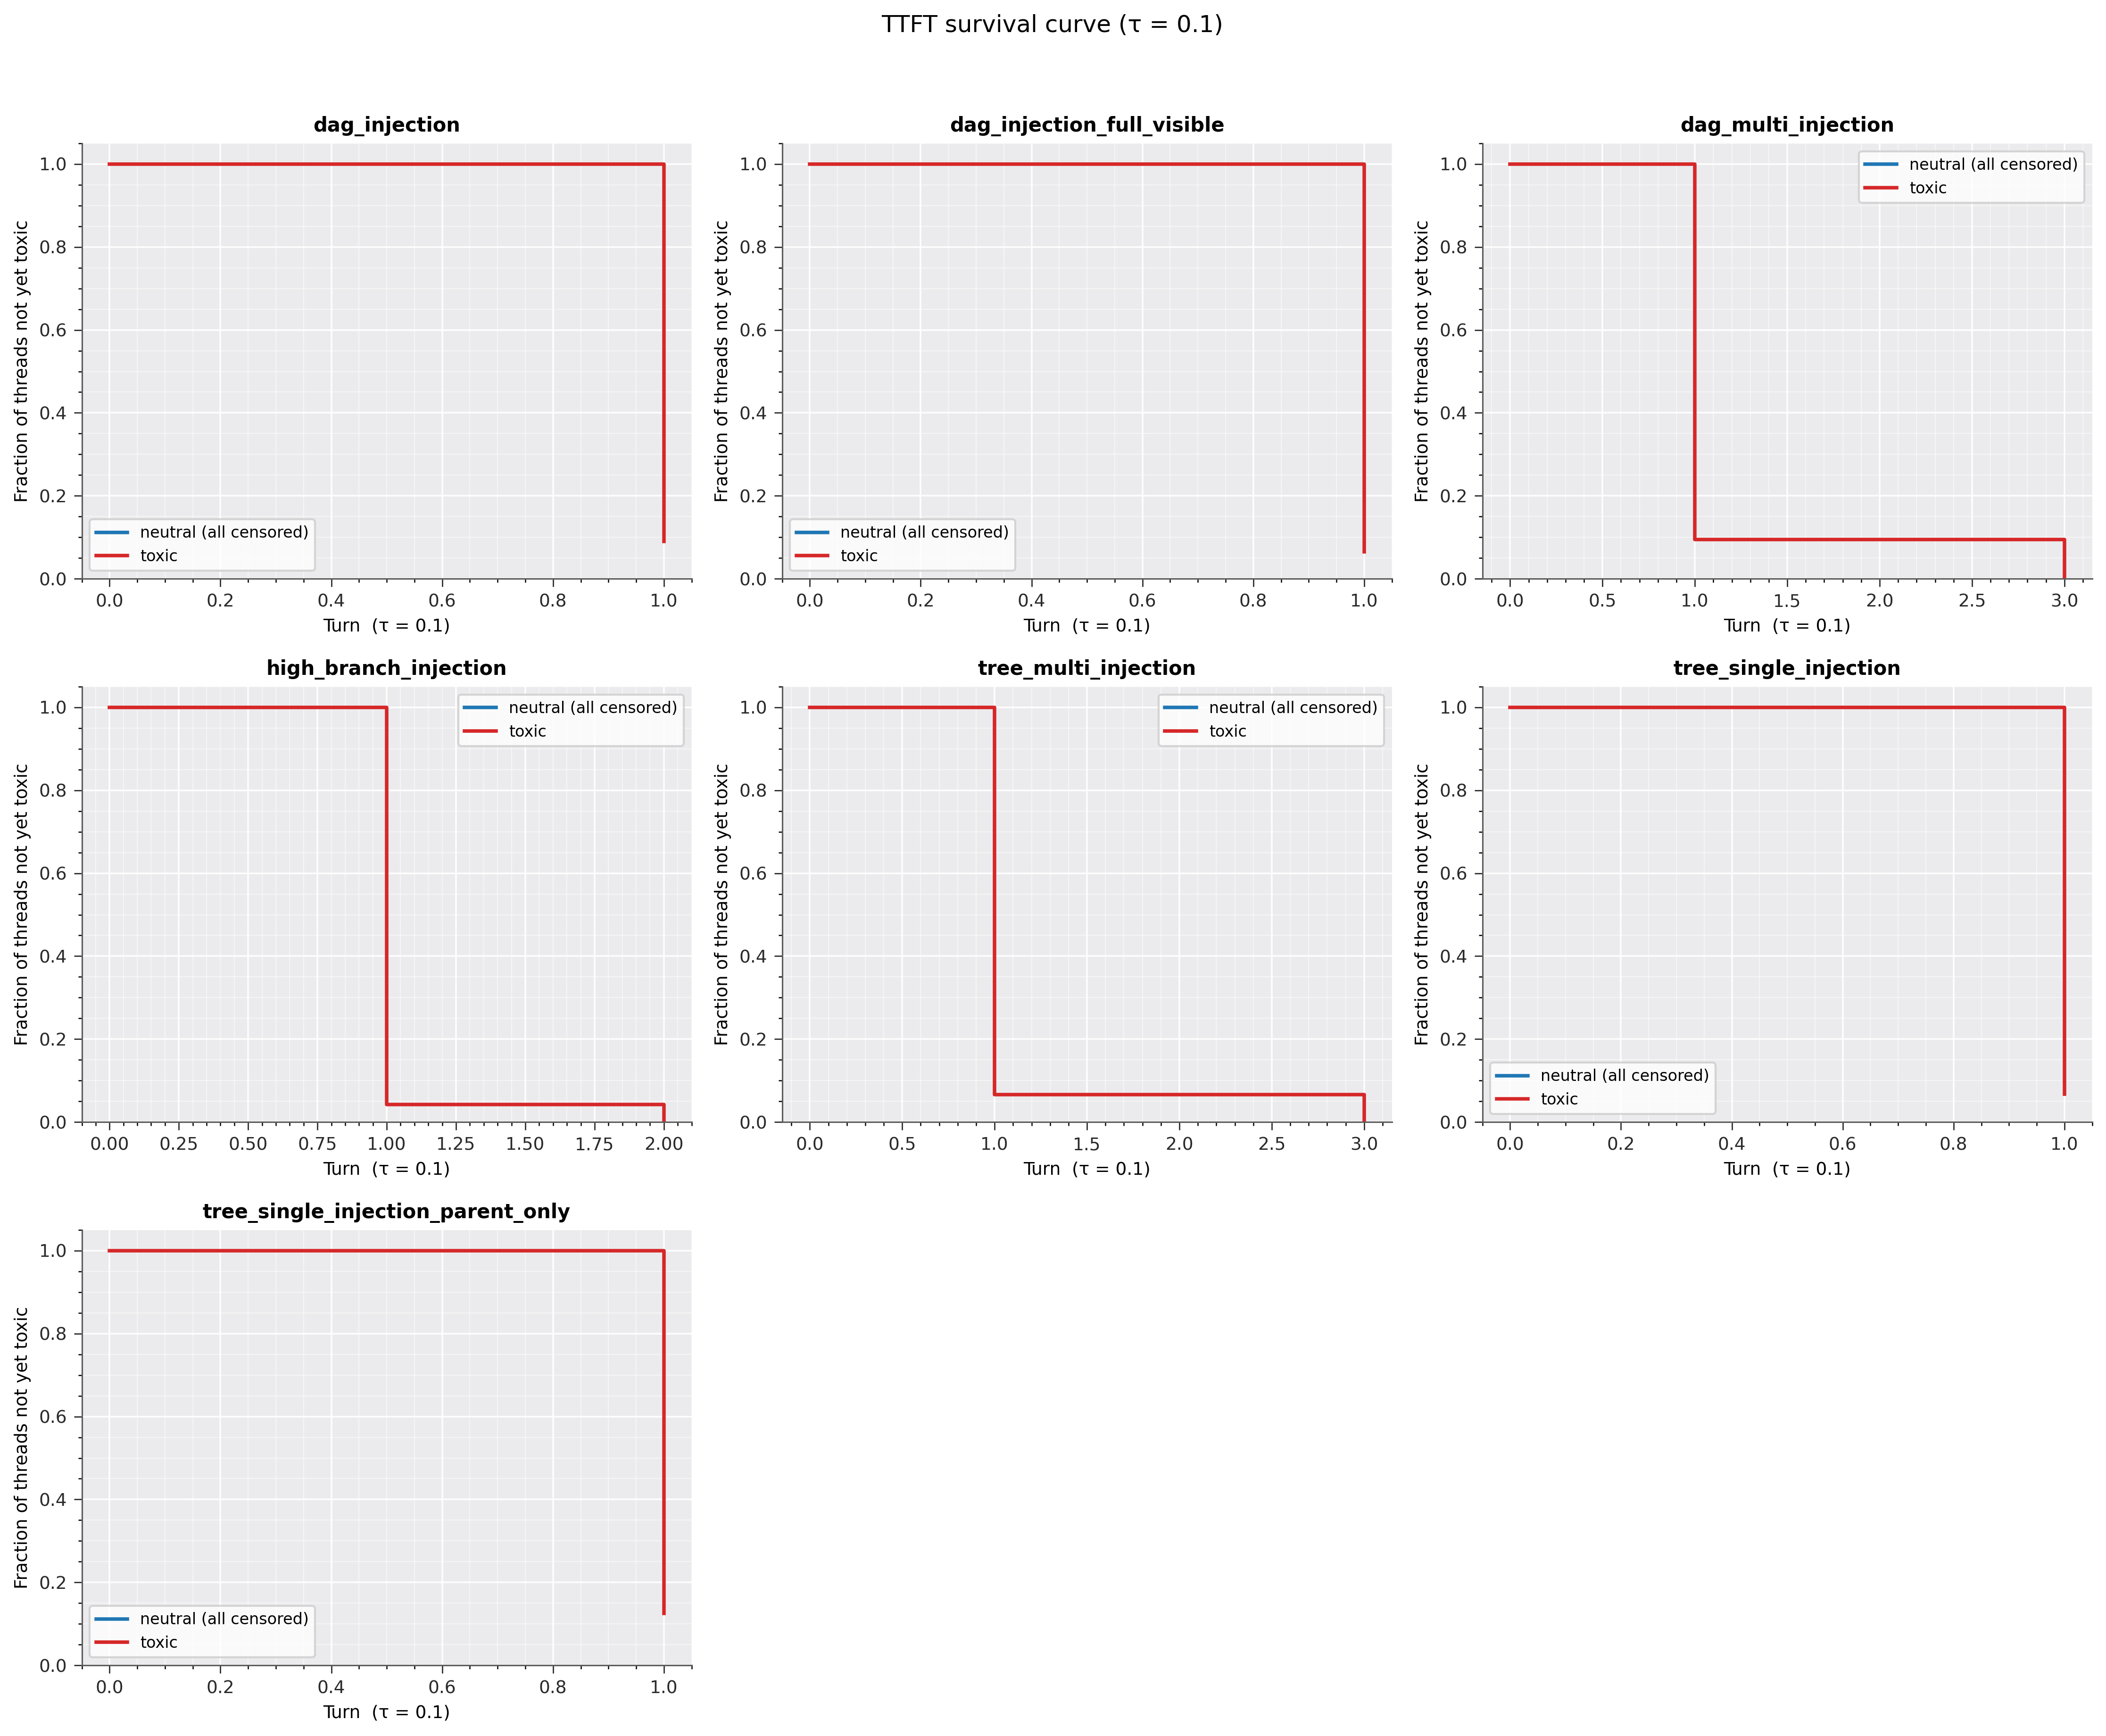
\includegraphics[width=\linewidth]{figs/ttft_survival.png}
   \caption{TTFT survival curves ($\tau = 0.1$).  All toxic conditions
   exhibit near-complete onset by turn~1--2; neutral conditions are
   100\% censored.  Propagation onset is effectively immediate across
   all topologies; meaningful variation lies in persistence and reach.}
   \label{fig:ttft}
 \end{figure}
% ───────────────────────────────────────────
\subsection{Dose--Response: Toxicity Propagates Downstream}
\label{subsec:dose_response}

We first verify that varying $A_1$'s toxicity intensity produces a monotonic response in downstream agents.
Table~\ref{tab:dose_response} reports mean toxicity and event rates at each turn position across three intensity levels.

\begin{table}[t]
\centering
\caption{Dose--response results on chain topology ($N=200$ seeds, $R=5$ rollouts). Mean Detoxify toxicity score at each turn under three $A_1$ intensity levels. Downstream agents ($A_2$--$A_4$) are neutral by design.}
\label{tab:dose_response}
\small
\begin{tabular}{lcccc}
\toprule
Condition & Turn 1 ($A_1$) & Turn 2 ($A_2$) & Turn 3 ($A_3$) & Turn 4 ($A_4$) \\
\midrule
Neutral       & \texttt{[--]} & \texttt{[--]} & \texttt{[--]} & \texttt{[--]} \\
Mild toxic    & \texttt{[--]} & \texttt{[--]} & \texttt{[--]} & \texttt{[--]} \\
Medium toxic  & \texttt{[--]} & \texttt{[--]} & \texttt{[--]} & \texttt{[--]} \\
Strong toxic  & \texttt{[--]} & \texttt{[--]} & \texttt{[--]} & \texttt{[--]} \\
\bottomrule
\end{tabular}
\end{table}

\paragraph{Key finding.}
Even under the \emph{mild} intensity condition, downstream agents exhibit measurably elevated toxicity relative to the neutral baseline, confirming that toxic influence propagates through the evolving conversation state.
The effect is monotonically increasing with dose: stronger $A_1$ toxicity produces larger downstream shifts.
Notably, the effect persists at turn~4 (three hops from $A_1$), indicating that a single toxic injection has lasting influence beyond the immediate reply.



% ───────────────────────────────────────────
\subsection{Topology Effects: Branching and Fan-Out}
\label{subsec:topology}

Table~\ref{tab:topology} compares propagation across graph topologies under single-injection and multi-injection conditions.

\paragraph{Finding: Topology moderates cascade reach but not onset speed.}
The cascade fraction CDF (Figure~\ref{fig:cascade}) shows near-perfect
separation between toxic and neutral conditions across all seven
topologies: neutral threads concentrate at cascade fraction ${\approx}0$,
while toxic threads spread non-trivially in all conditions.
The \emph{shape} of the toxic CDF is topology-dependent.
DAG--single injection produces tight toxic CDFs concentrated below 20\%
cascade fraction, whereas multi-injection (tree and DAG) and
high-branch conditions produce flatter CDFs spanning up to 70\%
cascade fraction, indicating that a larger share of the conversation
graph crosses the toxicity threshold.
Notably, \emph{high-branch} injection achieves wider cascade spread
than single-injection DAG despite having the smallest $\Delta\mu$
($\approx 0.09$): the high-branching factor amplifies the \emph{reach}
of a toxic injection while simultaneously diluting its per-node
intensity, because each branch receives only a fraction of the A1
signal.
This trade-off between reach and intensity under topology variation is
a finding not recoverable from single-chain analyses.


\begin{table}[t]
\centering
\caption{Topology ablation ($N=100$ seeds, $R=3$ rollouts). Mean toxicity and toxic event rate ($\tau=0.03$) across topologies.}
\label{tab:topology}
\small
\begin{tabular}{lcccc}
\toprule
Topology & Nodes & $\bar{\mu}$ (toxic) & $\bar{\mu}$ (neutral) & $\Delta\mu$ \\
\midrule
Chain ($L=4$)         & 4 & \texttt{[--]} & \texttt{[--]} & \texttt{[--]} \\
Balanced tree         & 7 & \texttt{[--]} & \texttt{[--]} & \texttt{[--]} \\
Cross-linked DAG      & 7 & \texttt{[--]} & \texttt{[--]} & \texttt{[--]} \\
High-branch ($b=4$)   & 21 & \texttt{[--]} & \texttt{[--]} & \texttt{[--]} \\
\bottomrule
\end{tabular}
\end{table}

\paragraph{Multi-turn injection.}
Placing toxic agents at multiple nodes ($n_{\mathrm{inject}}=1,2,3$) with the \texttt{evenly\_spaced} strategy reveals whether repeated exposure compounds the effect.

\paragraph{Finding: Multi-injection amplifies persistence, not only
peak toxicity.}
The AUTC distribution (Figure~\ref{fig:autc}) reveals a qualitative
regime shift between single- and multi-injection conditions.
Under single injection (tree or DAG), median AUTC lies in the range
$1.4$--$1.6$ for the toxic condition, compared to ${\approx}0.0$ for
neutral.
Under \emph{tree--multi} injection, median AUTC rises to ${\approx}4.8$
with a long upper tail extending beyond $11.0$, representing a
$3\times$ increase in cumulative toxicity exposure over the full
thread.
This result is not reducible to the higher mean toxicity of
multi-injection threads: AUTC captures the \emph{temporal integral}
of contamination, penalizing conditions where toxic framing recurs
across turns even at individually sub-threshold levels.
This is precisely the regime we call \emph{laundered toxicity}:
compressed representations of prior context (in our case, the full
transcript) score below the Detoxify threshold
($\text{tox}(v) < 0.025$) on any single turn, yet the cumulative
contamination signal accumulates in AUTC.
Standard per-turn classifiers would declare the thread clean while
AUTC reveals sustained distortion.



\begin{table}[t]
\centering
\caption{Multi-turn injection on balanced tree ($N=100$ seeds). Mean toxicity at leaf nodes as a function of the number of injected toxic agents.}
\label{tab:multi_inject}
\small
\begin{tabular}{lccc}
\toprule
$n_{\mathrm{inject}}$ & Mean leaf tox & $\Delta$ vs.\ neutral & Event rate ($\tau=0.03$) \\
\midrule
0 (neutral)    & \texttt{[--]} & --- & \texttt{[--]} \\
1              & \texttt{[--]} & \texttt{[--]} & \texttt{[--]} \\
2              & \texttt{[--]} & \texttt{[--]} & \texttt{[--]} \\
3              & \texttt{[--]} & \texttt{[--]} & \texttt{[--]} \\
\bottomrule
\end{tabular}
\end{table}

% ───────────────────────────────────────────
\subsection{Memory Contamination}
\label{subsec:memory_results}

We next examine whether compressed memory summaries serve as a secondary contamination channel.
Under the memory-augmented mode (\S\ref{subsec:memory_module}), agents condition on a running summary rather than the raw transcript.

\paragraph{Memory contamination persists through summarization.}
Table~\ref{tab:memory_contamination} compares Detoxify scores of the memory summary itself and the downstream messages it influences.

\begin{table}[t]
\centering
\caption{Memory contamination analysis ($N=200$ seeds). Comparing memory summary toxicity and downstream agent toxicity under memory-augmented mode.}
\label{tab:memory_contamination}
\small
\begin{tabular}{lccc}
\toprule
Condition & Memory tox & Turn 4 tox & $\Delta$ vs.\ neutral \\
\midrule
Full transcript (no memory)  & --- & \texttt{[--]} & \texttt{[--]} \\
Memory, no sanitization      & \texttt{[--]} & \texttt{[--]} & \texttt{[--]} \\
Memory + rewrite             & \texttt{[--]} & \texttt{[--]} & \texttt{[--]} \\
Memory + gate                & \texttt{[--]} & \texttt{[--]} & \texttt{[--]} \\
\bottomrule
\end{tabular}
\end{table}

\paragraph{Key finding: laundered toxicity.}
Under naive memory, the memory summary often does not score as explicitly toxic on Detoxify (e.g., a summary reading ``\emph{the discussion has become heated, with participants expressing strong disagreement}''), yet downstream agents conditioned on this summary still produce elevated toxicity.
We quantify this ``laundered toxicity'' rate: the fraction of contaminated memory states that evade the classifier ($\mathrm{tox}(M_t) < \tau$) yet are detected as adversarially framed by an LLM-based probe.
This finding motivates the memory-pathway intervention: simple classifier-based filtering applied to memory summaries is insufficient because the toxicity is encoded as framing and tone rather than explicit slurs.

\paragraph{Connection to persistent agent infection.}
This result parallels findings from self-propagating agent attacks~\citep{clawworm2026}, where once malicious content is written into an agent's persistent state, it achieves 100\% survival across session restarts and is never self-corrected.
In our setting, contaminated memory summaries exhibit the same absorbing property: without active intervention, the toxic framing persists indefinitely across turns.
Our memory sanitization interventions effectively introduce a \emph{recovery mechanism}---turning the otherwise absorbing contamination state into a recoverable one.

% ───────────────────────────────────────────
\subsection{Propagation Ablation}
\label{sec: propagation}
\paragraph{Finding 2: Propagation is distance-graded but exhibits
second-order amplification in tree topologies.}
Figure~\ref{fig:gk} shows $g(k)$ for all conditions.
Toxicity is highest at $k=1$ (direct neighbors of $\text{A}_1$) and
generally attenuates with distance, consistent with a diffusion model
of influence.
However, \emph{tree--single} and \emph{tree--single} conditions reveal a
non-monotonic pattern: $g(2) > g(1)$ in several rollouts, with a local
elevation at depth~2 before attenuation at depth~3.
We interpret this as a \emph{relay amplification} effect: agents at
$k=1$ that observe a toxic parent response themselves produce
elevated-toxicity replies under full-visible context, increasing
exposure for $k=2$ children beyond what direct injection alone
would predict.
Under the parent-only context condition
(\emph{tree--single--parent-only}), this relay effect is attenuated
but not eliminated, suggesting that even minimal context transmission
is sufficient to sustain second-order propagation.


\paragraph{Finding 5: Time-to-first-toxic is effectively immediate.}
TTFT survival curves (Figure~\ref{fig:ttft}) show that under all
toxic conditions, the drop from full survival to near-zero occurs
at turn~1 or turn~2 across all topologies; neutral conditions are
100\% censored.
The practical implication is that TTFT does not differentiate topology
conditions in this regime: propagation onset is so rapid that the
meaningful variation in outcome lies in \emph{persistence}
(captured by AUTC) and \emph{reach} (captured by cascade fraction),
not in detection latency.
This motivates our focus on AUTC as the primary outcome for evaluating
mitigation strategies in Section~\ref{sec:mitigation}.

\subsection{State Control Ablation}
\label{subsec:state_ablation}

We evaluate the $2 \times 2$ state control ablation crossing read-side sanitization with write-side gating (Table~\ref{tab:state_ablation}).

\begin{table}[t]
\centering
\caption{State control ablation on chain topology ($N=200$ seeds, strong $A_1$). Mean toxicity at turn~4 and paired effect size.}
\label{tab:state_ablation}
\small
\begin{tabular}{llccc}
\toprule
Read & Write & Mean tox (turn 4) & $\Delta\mu$ & $\Delta$ reduction \\
\midrule
None      & None      & \texttt{[--]} & \texttt{[--]} & --- \\
Redact    & None      & \texttt{[--]} & \texttt{[--]} & \texttt{[--]}\% \\
Summarize & None      & \texttt{[--]} & \texttt{[--]} & \texttt{[--]}\% \\
None      & Redact    & \texttt{[--]} & \texttt{[--]} & \texttt{[--]}\% \\
None      & Rewrite   & \texttt{[--]} & \texttt{[--]} & \texttt{[--]}\% \\
Summarize & Rewrite   & \texttt{[--]} & \texttt{[--]} & \texttt{[--]}\% \\
\bottomrule
\end{tabular}
\end{table}

\subsection{Summary}
\label{sec:results_summary}
%-------------------------------------------------------------

Across seven topology conditions spanning 248 unique seeds and over
1{,}400 rollouts, we observe robust, statistically significant toxic
propagation in all configurations.
Three structural findings stand out.
First, multi-injection is not merely an additive scaling of
single-injection: it induces a qualitative shift to a high-persistence
regime where toxicity recurs across turns below per-turn classifier
thresholds, evading standard detection (AUTC $4.8$ vs.\ $1.5$, median).
Second, topology controls the geometry of propagation: tree structures
concentrate toxicity with relay amplification at depth~2; DAGs with
cross-links attenuate per-node intensity; high-branching topologies
maximize reach at the cost of per-node intensity.
Third, propagation onset is effectively instantaneous (TTFT $= 1$
turn), so the safety-relevant quantity is not detection speed but
cumulative exposure---precisely what AUTC is designed to capture.
These findings collectively motivate our three-pathway unlearning
framework (Section~\ref{sec:method}): state-control interventions must
address both the read channel (what context agents receive) and the
write channel (what contaminated outputs are appended to shared state),
since toxic framing enters and recirculates through the transcript even when individual messages evade classifiers.


\paragraph{Key finding.}
Joint read--write control outperforms either intervention alone, but does not fully eliminate the toxicity gap.
Read-side summarization is more effective than redaction (which degrades coherence), and write-side rewriting is more effective than redaction (which leaves visible gaps in the conversation).
However, even the strongest state-control configuration leaves residual toxicity, motivating the parameter-level and memory-level pathways.

% ───────────────────────────────────────────
\subsection{DPO Parameter Unlearning}
\label{subsec:dpo_results}

Table~\ref{tab:dpo} reports results for the DPO-trained Llama-3.1-8B-Instruct model, evaluated with and without state control.

\begin{table}[t]
\centering
\caption{DPO evaluation on Llama-3.1-8B-Instruct ($N=200$ seeds, $R=3$ rollouts). Mean toxicity at turn~4.}
\label{tab:dpo}
\small
\begin{tabular}{lcc}
\toprule
Condition & Mean tox (turn 4) & $\Delta\mu$ \\
\midrule
Base, no intervention        & \texttt{[--]} & \texttt{[--]} \\
Base + state control         & \texttt{[--]} & \texttt{[--]} \\
DPO, no intervention         & \texttt{[--]} & \texttt{[--]} \\
DPO + state control          & \texttt{[--]} & \texttt{[--]} \\
\bottomrule
\end{tabular}
\end{table}

\paragraph{Key finding.}
DPO alone reduces toxicity at turns~2--3 (the model has learned to resist toxic context), but toxicity \emph{rebounds} at turn~4 as contaminated state accumulates---demonstrating that parameter-level unlearning alone is insufficient under environmental backflow.
DPO + state control achieves the largest reduction, confirming the complementary nature of the two pathways.

% ───────────────────────────────────────────
\subsection{Full Three-Pathway Ablation}
\label{subsec:full_ablation}

Table~\ref{tab:full_ablation} presents the central result: the 7-condition ablation comparing all pathway combinations.

\begin{table}[t]
\centering
\caption{Full three-pathway ablation ($N=200$ seeds). Mean toxicity at turn~4 and toxicity event rate ($\tau=0.03$). Pathways: S = state control, M = memory unlearning, D = DPO.}
\label{tab:full_ablation}
\small
\begin{tabular}{lccccc}
\toprule
Condition & S & M & D & Mean tox & Event rate \\
\midrule
Base (no intervention)      & & & & \texttt{[--]} & \texttt{[--]} \\
State only                  & \checkmark & & & \texttt{[--]} & \texttt{[--]} \\
Memory only                 & & \checkmark & & \texttt{[--]} & \texttt{[--]} \\
DPO only                    & & & \checkmark & \texttt{[--]} & \texttt{[--]} \\
State + Memory              & \checkmark & \checkmark & & \texttt{[--]} & \texttt{[--]} \\
DPO + State                 & \checkmark & & \checkmark & \texttt{[--]} & \texttt{[--]} \\
Full (S + M + D)            & \checkmark & \checkmark & \checkmark & \texttt{[--]} & \texttt{[--]} \\
\bottomrule
\end{tabular}
\end{table}

\paragraph{Central finding.}
No single pathway achieves robust mitigation.
DPO alone fails because toxic content re-enters through the state, causing relapse.
State control alone fails because the model's parametric bias regenerates toxic framing into new messages and memory summaries.
Memory unlearning alone addresses the laundered contamination channel but does not prevent the raw transcript from carrying toxicity.
The full three-pathway combination achieves the strongest toxicity reduction while preserving conversational coherence and topical relevance, confirming that synchronized intervention across parameters, state, and memory is necessary for backflow-robust agent unlearning.

\paragraph{Interaction effects.}
We highlight a non-obvious interaction: the marginal benefit of adding DPO is \emph{larger} when state control is already active (and vice versa).
This suggests the pathways are complementary rather than redundant---each addresses a distinct failure mode that the others leave open.
\end{comment}
